% Intro on the section
This section describes the data management layer for this project, i.e. how data is managed, versioned, etc. The main \gls{DBMS} technology used in this is Delta Lake, and to understand it Section \ref{subsec:history_DBMS} revises the problems that technologies aimed to solve, and the limitations of these systems. The chapter is complemented with Section \ref{subsec:delta_lake_access} which explains how to access Delta Lake and introduces delta-rs.

\subsection{Brief history of \glsfmtlongpl{DBMS}}
\label{subsec:history_DBMS}

In recent years the rise of Big Data, large volumes of various structured and unstructured data types at a high velocity, has shown an incredible potential but it has also posed several challenges \cite{penceWhatBigData2014}. These mostly impact the software architecture that needs to deal with these issues, which led to an evolution of these technologies \cite{gortonDistributionDataDeployment2015}. Delta Lake \cite{armbrustDeltaLakeHighperformance2020}, is one of the most recent iterations of this evolution process, but to understand the tool, it is necessary to understand the challenges, starting from the beginning of the data management evolution.

Before Big Data, companies already wanted to gain insights from their data sources using an automated workflow. Here is where \gls{ETL} and relational databases first came into use. An \gls{ETL} pipeline as the name suggests:
\begin{enumerate}
    \item Extracts data from \glspl{API} or other company's data sources.
    \item Transforms data by removing errors or absent fields, standardizes the format to match the database, and validates the data to verify its correctness.
    \item Loads it into a relational database (e.g. MySQL).
\end{enumerate} 

\begin{figure}[!ht]
    \begin{center}
      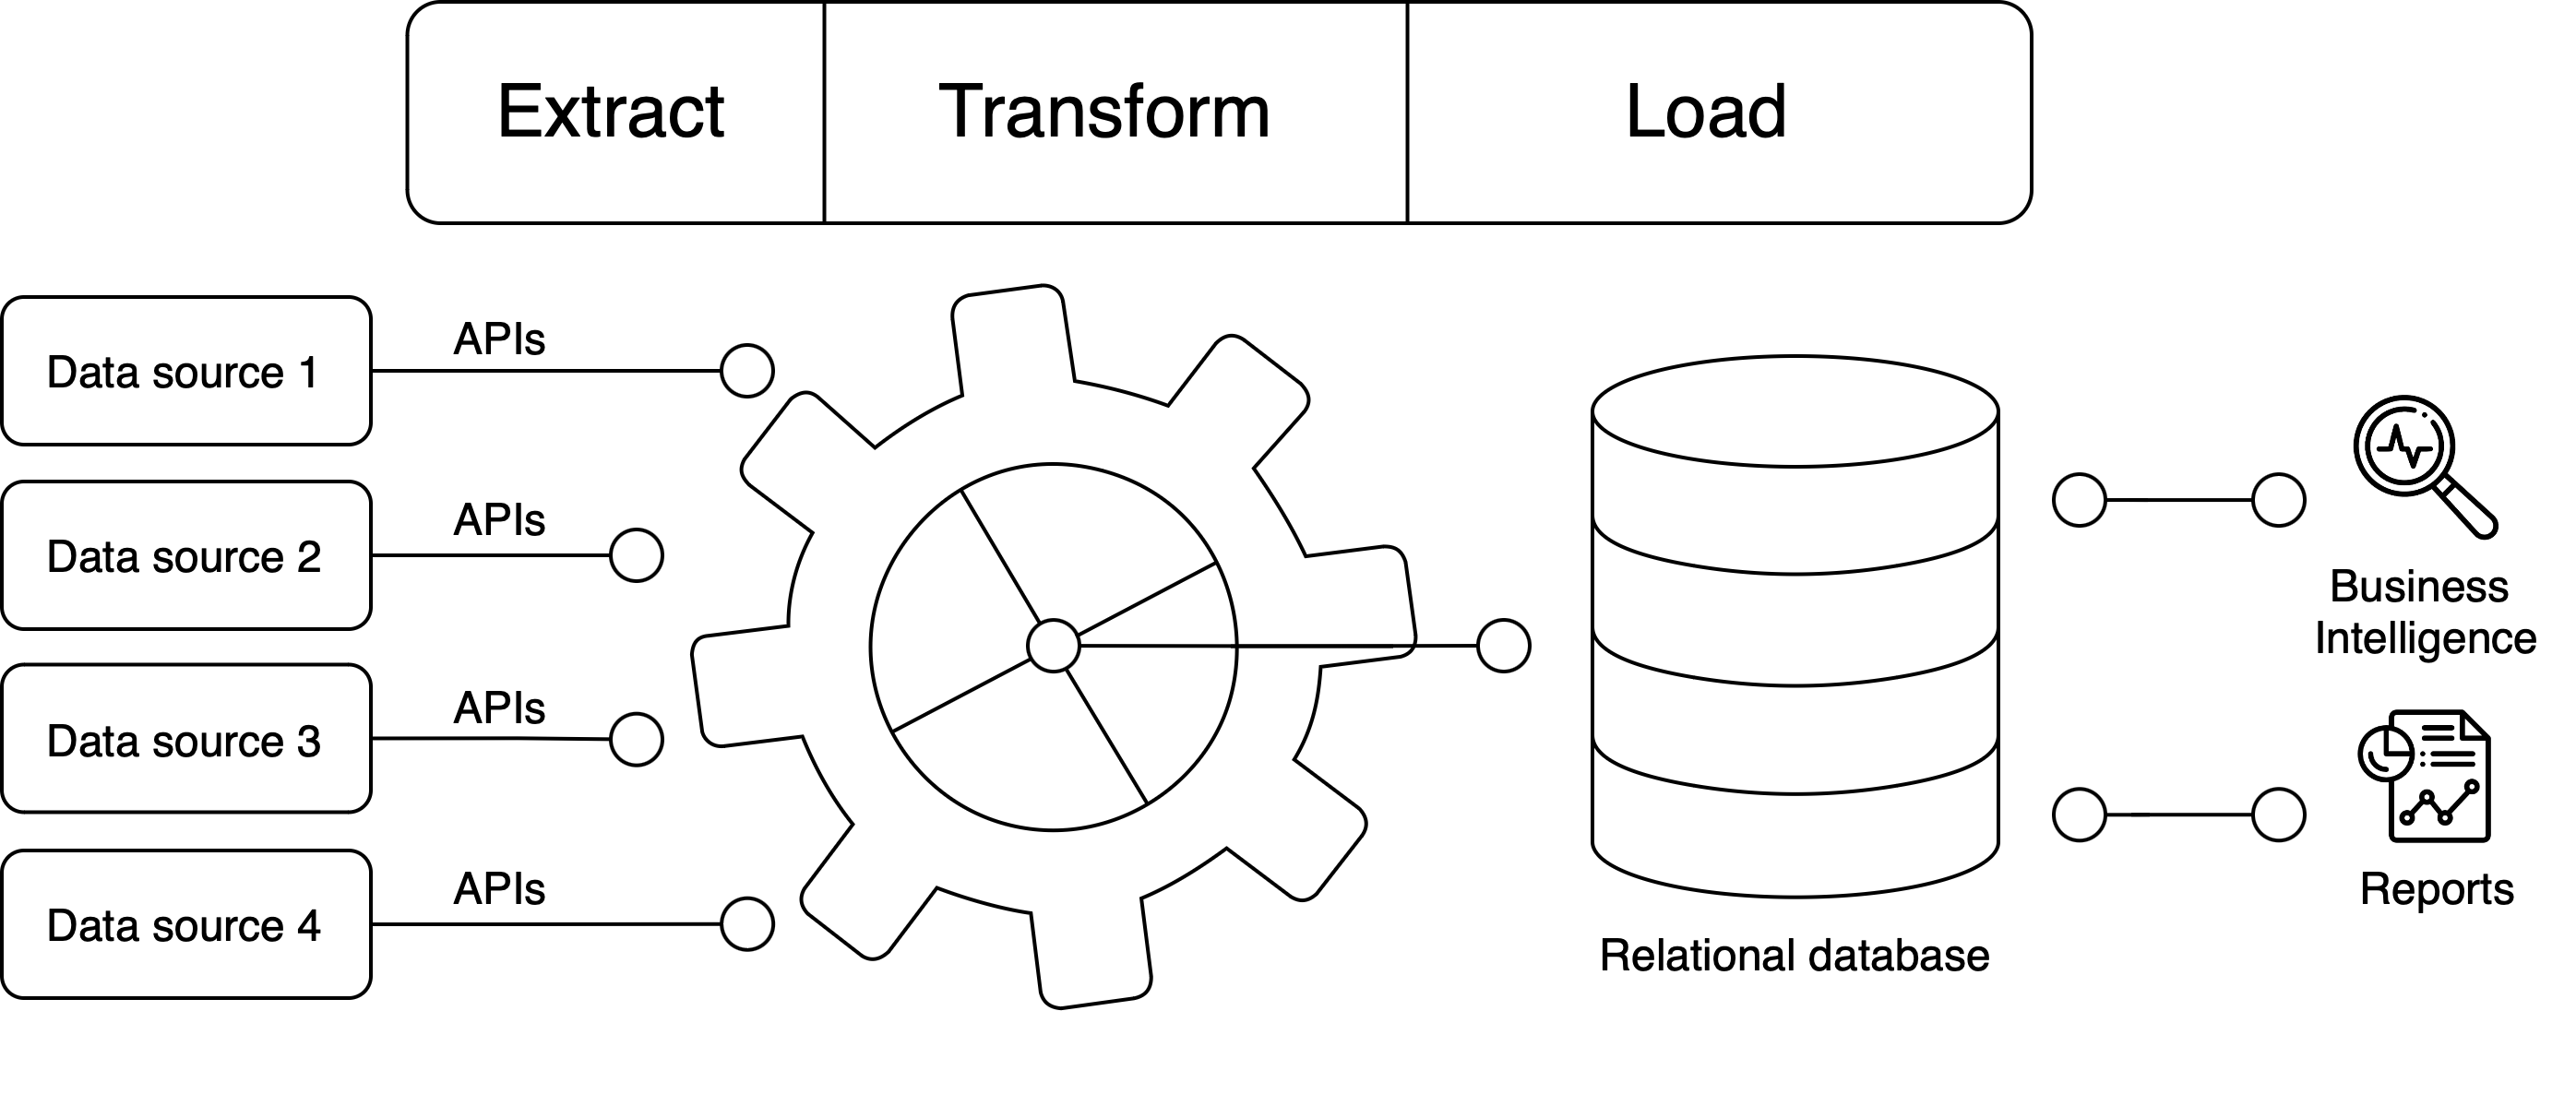
\includegraphics[width=\textwidth]{figures/2-background/DeltaLake_evolution-ETL+DB.png}
    \end{center}
    \caption{Simple \gls{ETL} system with a relational database}
    \label{fig:ETL+DB}
\end{figure}
% Figure inspired by AltexSoft video \cite{altexsoftHowDataEngineering2021}

This type of workflow, represented in Figure \ref{fig:ETL+DB}, enabled companies to obtain \gls{BI} insights and data reports on the company's data. The main limitation of this system sat in its limited capability of creating reports or \gls{BI} insights based on data sitting on multiple tables. These types of requests are called analytical queries, and while they might run less often than simpler queries are still crucial for making data-driven decisions (e.g. determining the region that sold more product units in the last year).

When the need to compute analytical queries rose, more complex \gls{DBMS} substituted the simple relational databases, optimizing for running business-centric complex analytical queries. These systems are called \gls{OLAP}, and its prime example example is the data warehouse.

\begin{figure}[!ht]
    \begin{center}
      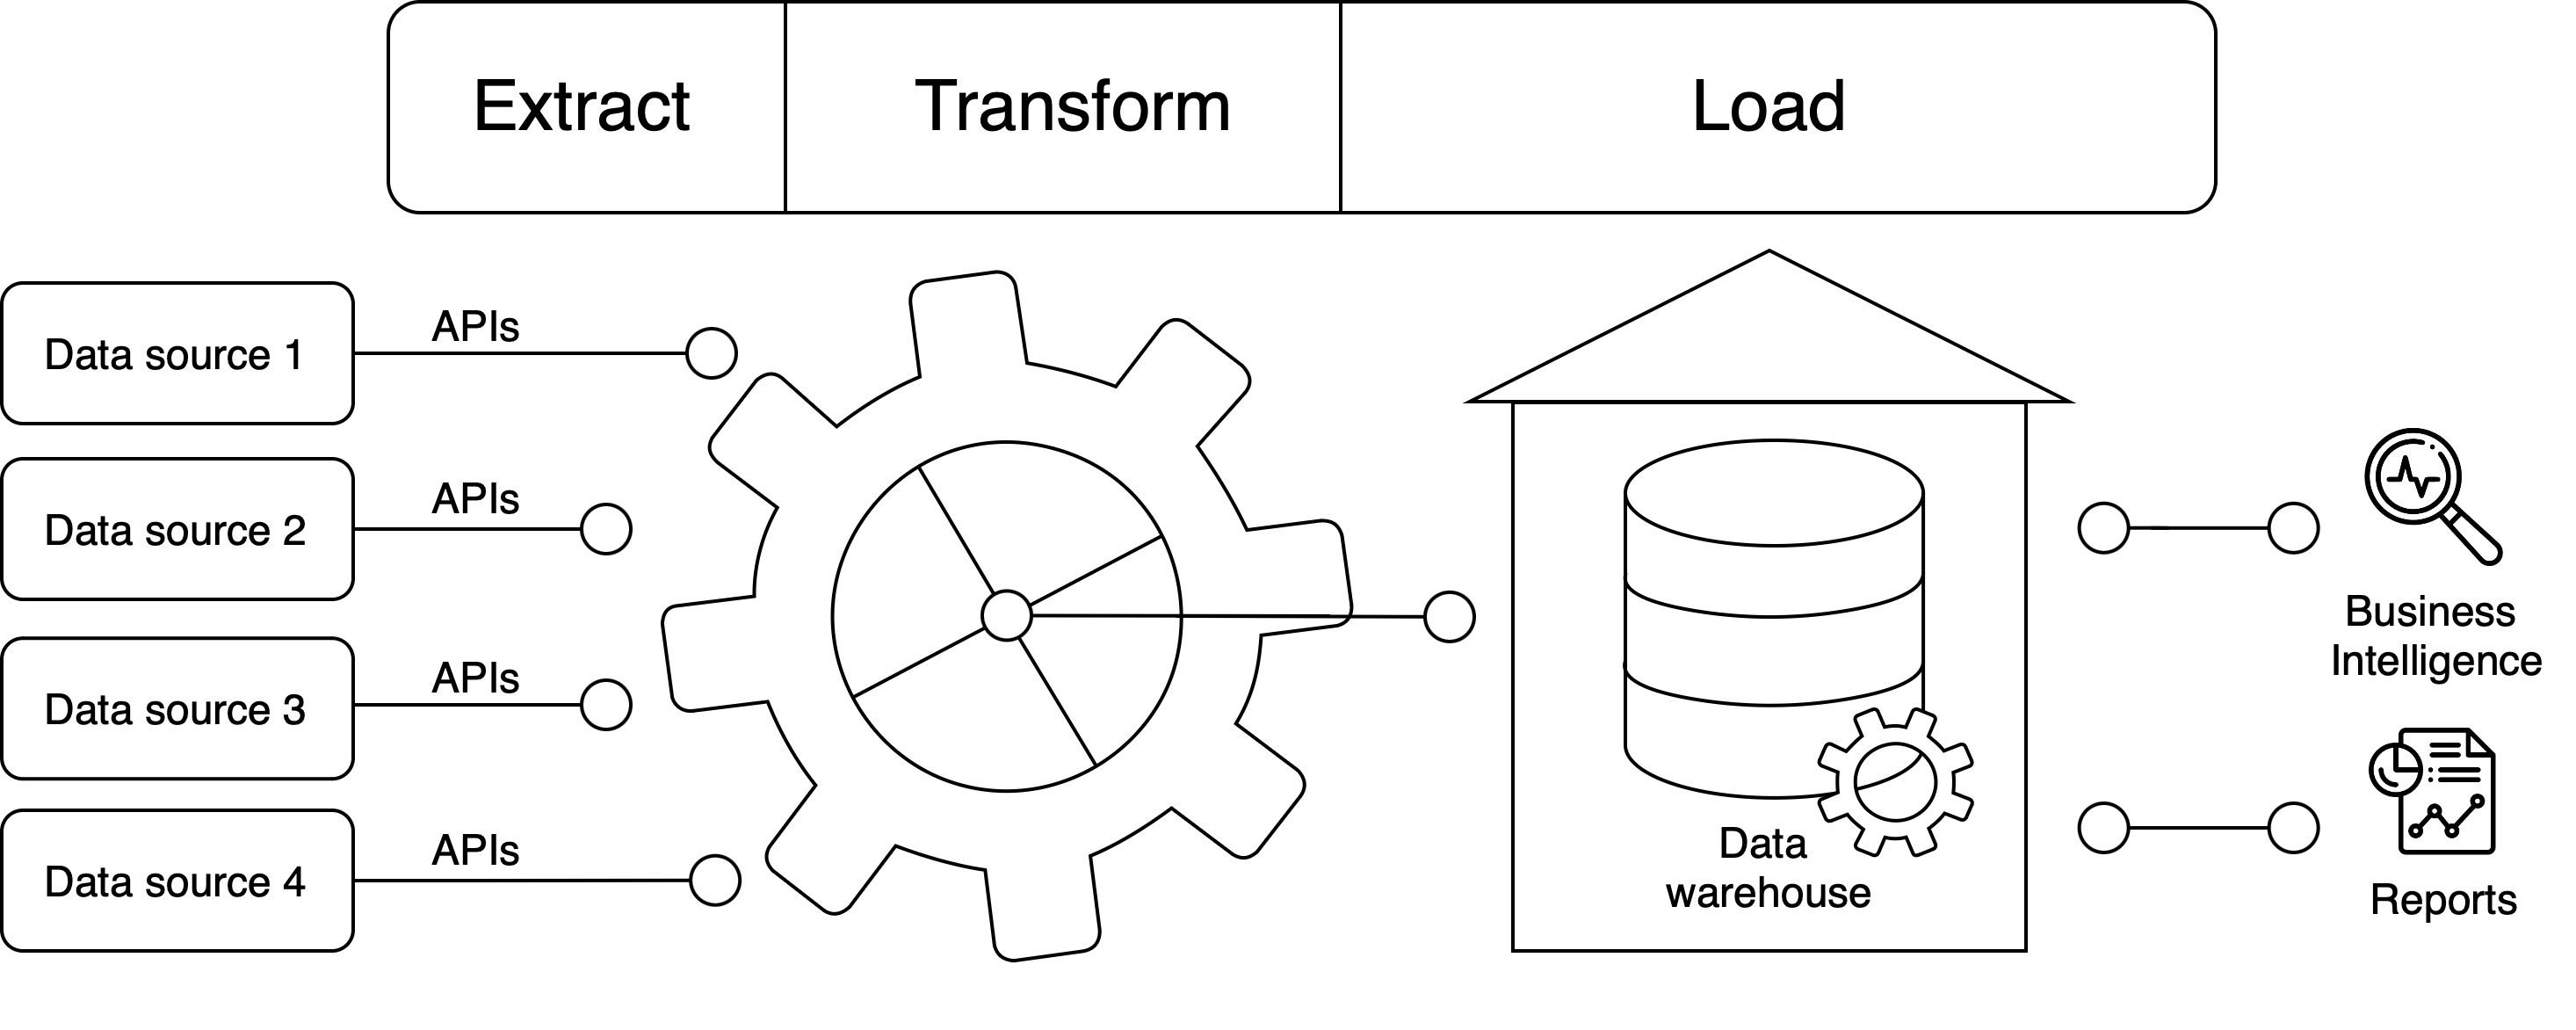
\includegraphics[width=\textwidth]{figures/2-background/DeltaLake_evolution-ETL+DW.png}
    \end{center}
    \caption{\gls{ETL} system with a data warehouse}
    \label{fig:ETL+DW}
\end{figure}

A data warehouse workflow, visualized in Figure \ref{fig:ETL+DW}, enables larger quantities of data to be computed and analyzed. Data warehouses enable \gls{BI} and Reports that consider all data sources and can join multiple tables efficiently. This type of \gls{DBMS} still keeps a relational database key features, such as \gls{ACID} transactions and data versioning.

Over time, the rapidly growing amount of unstructured data (also called Big Data, e.g. images, and videos) created new needs within companies, that wanted to take advantage of this new data. Data warehouses were unfit to solve this problem as they only supported structured data. Furthermore, storing large quantities of data in data warehouses is expensive and does not support any type of \gls{AI}/\gls{ML} workflow.

These issues were tackled by a new paradigm called Data Lake (Figure \ref{fig:ELT+DL}). Data Lakes are based on a low-cost object storage system (Section \ref{subsec:file_vs_obj_vs_block}) that consists of a flat structure where all data is loaded after extraction. In data lakes the architecture structure changes as data is first loaded into the data lake and only after transformed. This paradigm is called \gls{ELT}. Transformations are customizable for specific applications, e.g. \gls{BI} and reports using a Data warehouse, an \gls{AI}/\gls{ML} analysis.

\begin{figure}[!ht]
    \begin{center}
      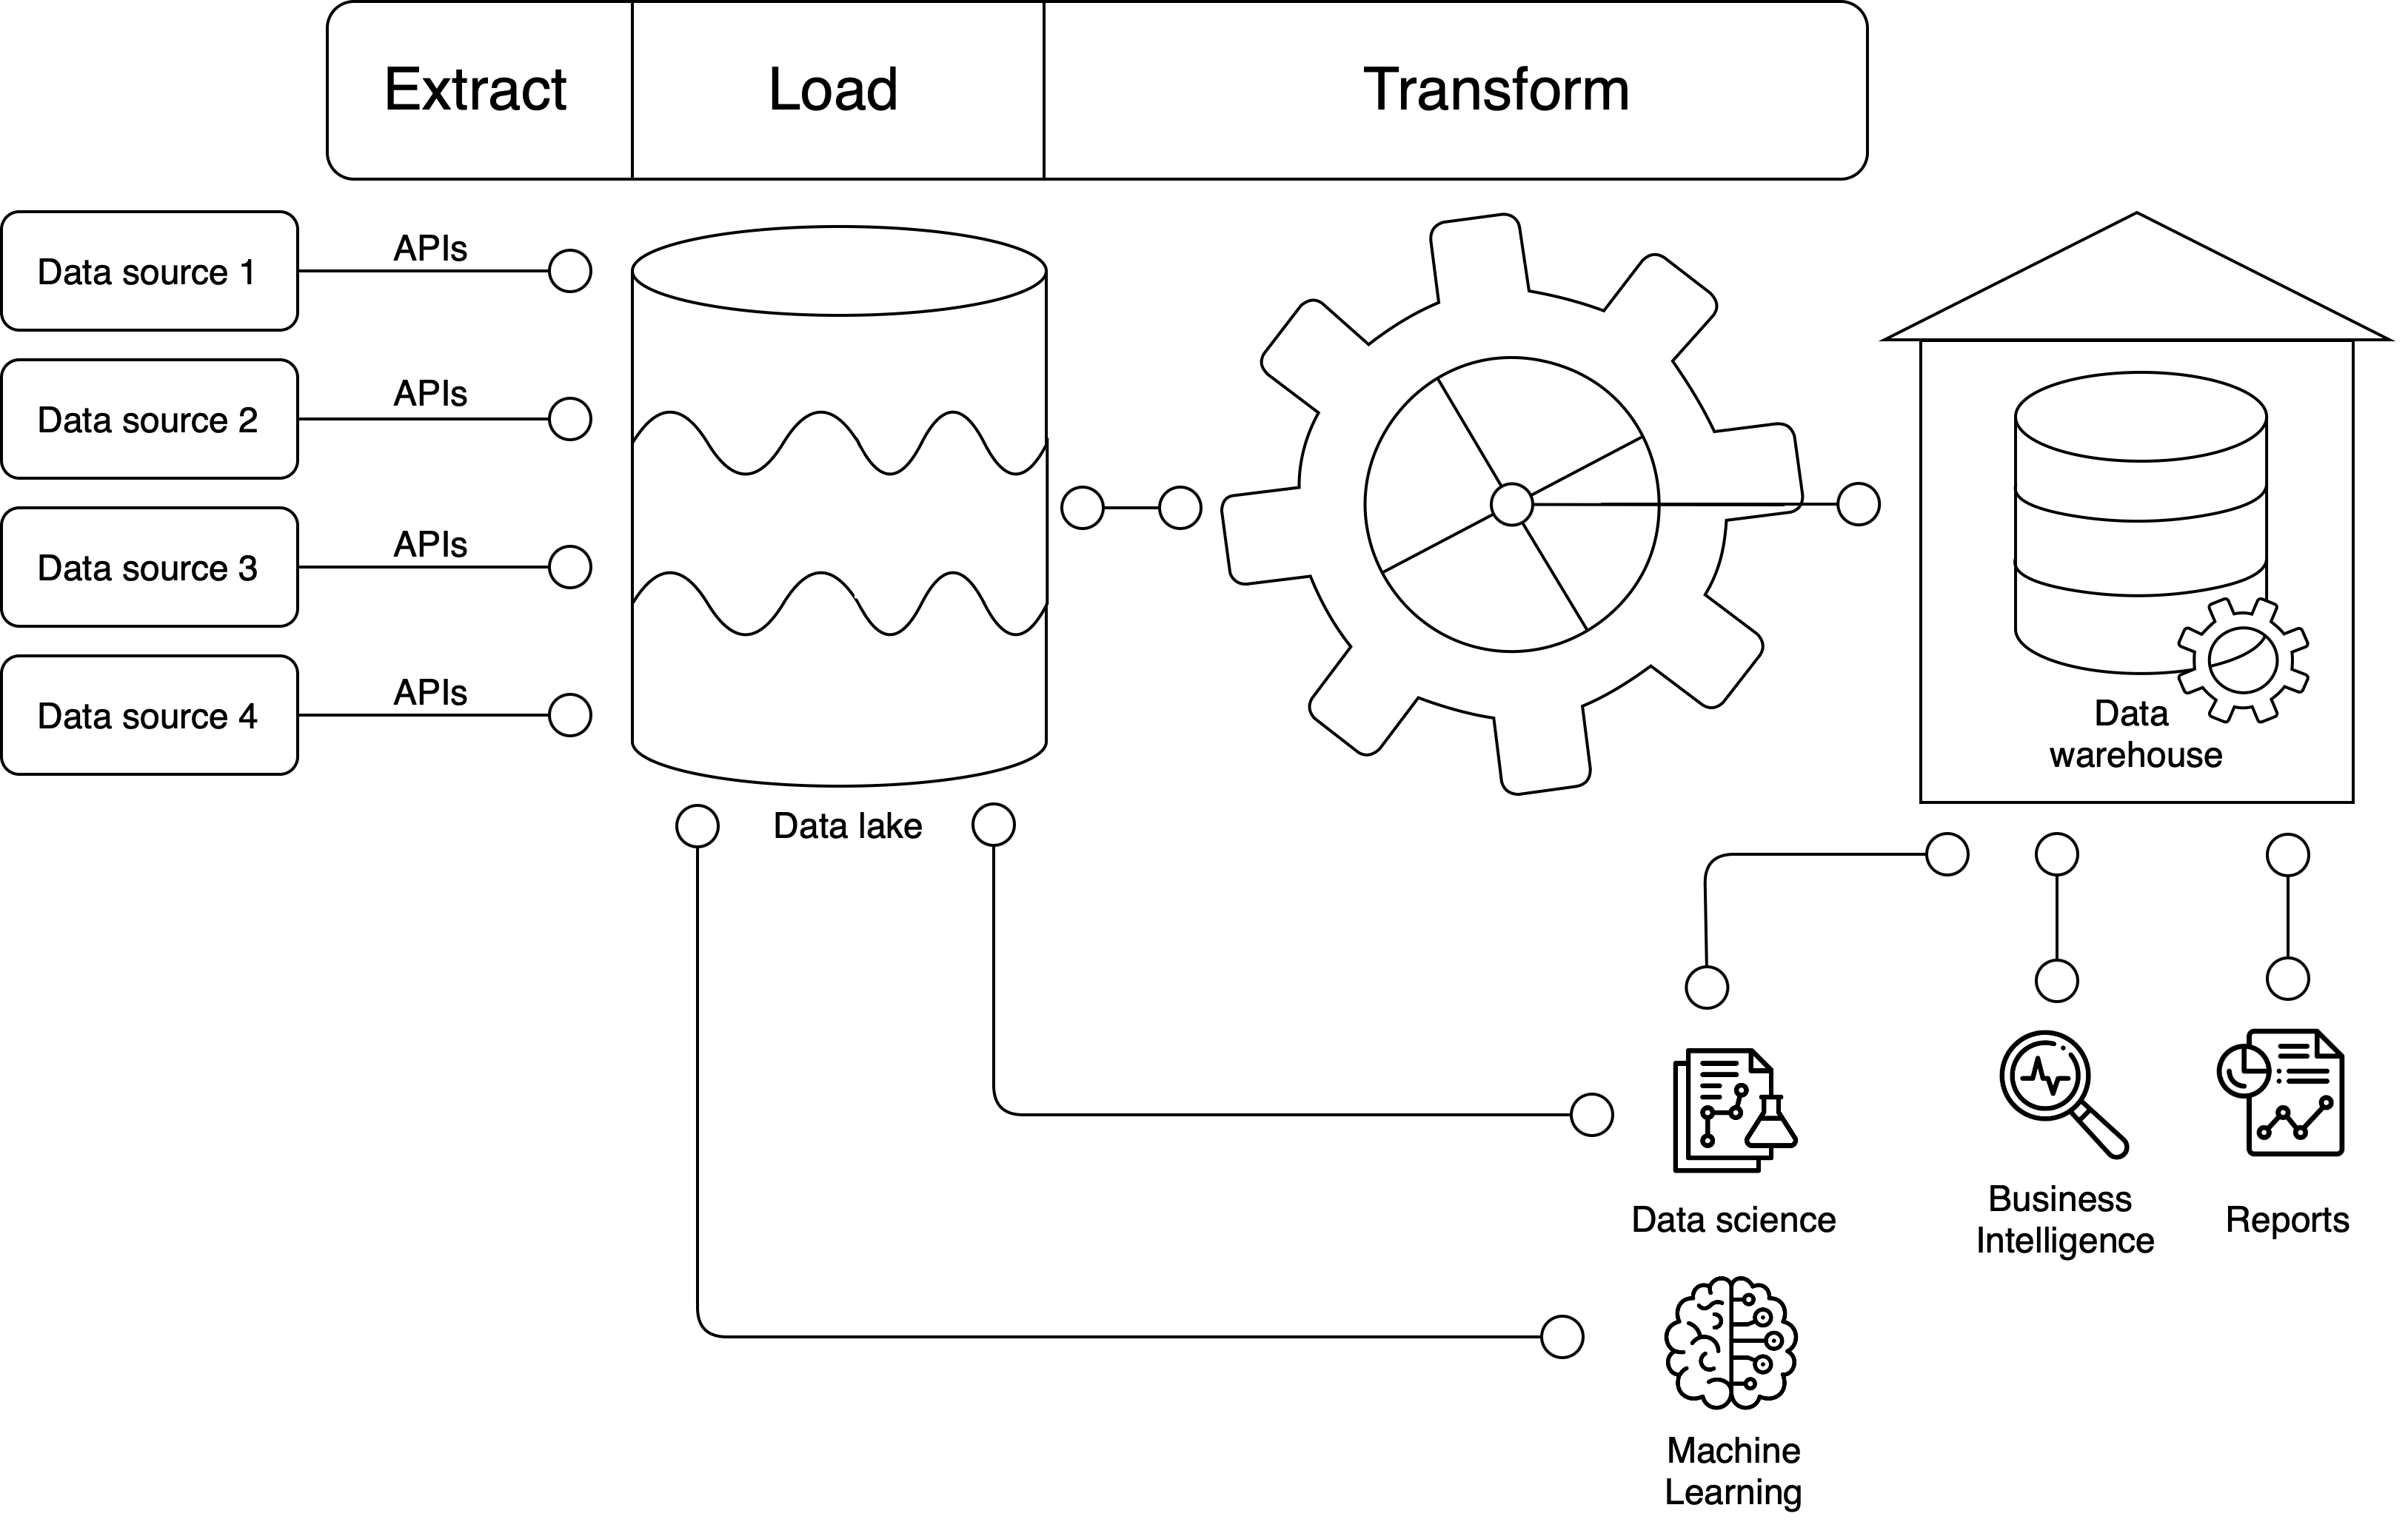
\includegraphics[width=\textwidth]{figures/2-background/DeltaLake_evolution-ELT+DL.png}
    \end{center}
    \caption{\gls{ELT} system with a data lake}
    \label{fig:ELT+DL}
\end{figure}

This architecture reduces storage costs but also increases the system complexity. Higher complexity is typically related to higher costs, as system maintenance is more costly and can lead to a larger number of issues. Additionally, since data lake cannot be queried directly with \gls{BI} queries or requesting business reports, this leads to the need to still maintain a data warehouse (as in Figure \ref{fig:ELT+DL}). This ultimately leads to higher costs to maintain the multiple storages for the same data. The system also suffers from timeliness due to this lengthy pipeline, as the data needs to go through many steps before it is available in the data warehouse. 

These issues outlined that data lakes were not a drop-in replacement for data warehouses, as they served a different purpose and suffered from different issues. This generated the need to have a system that could have data warehouses \gls{ACID} and data management capabilities while being able to support unstructured data. The solution was a new architecture, the data lakehouse. 

\begin{figure}[!ht]
    \begin{center}
      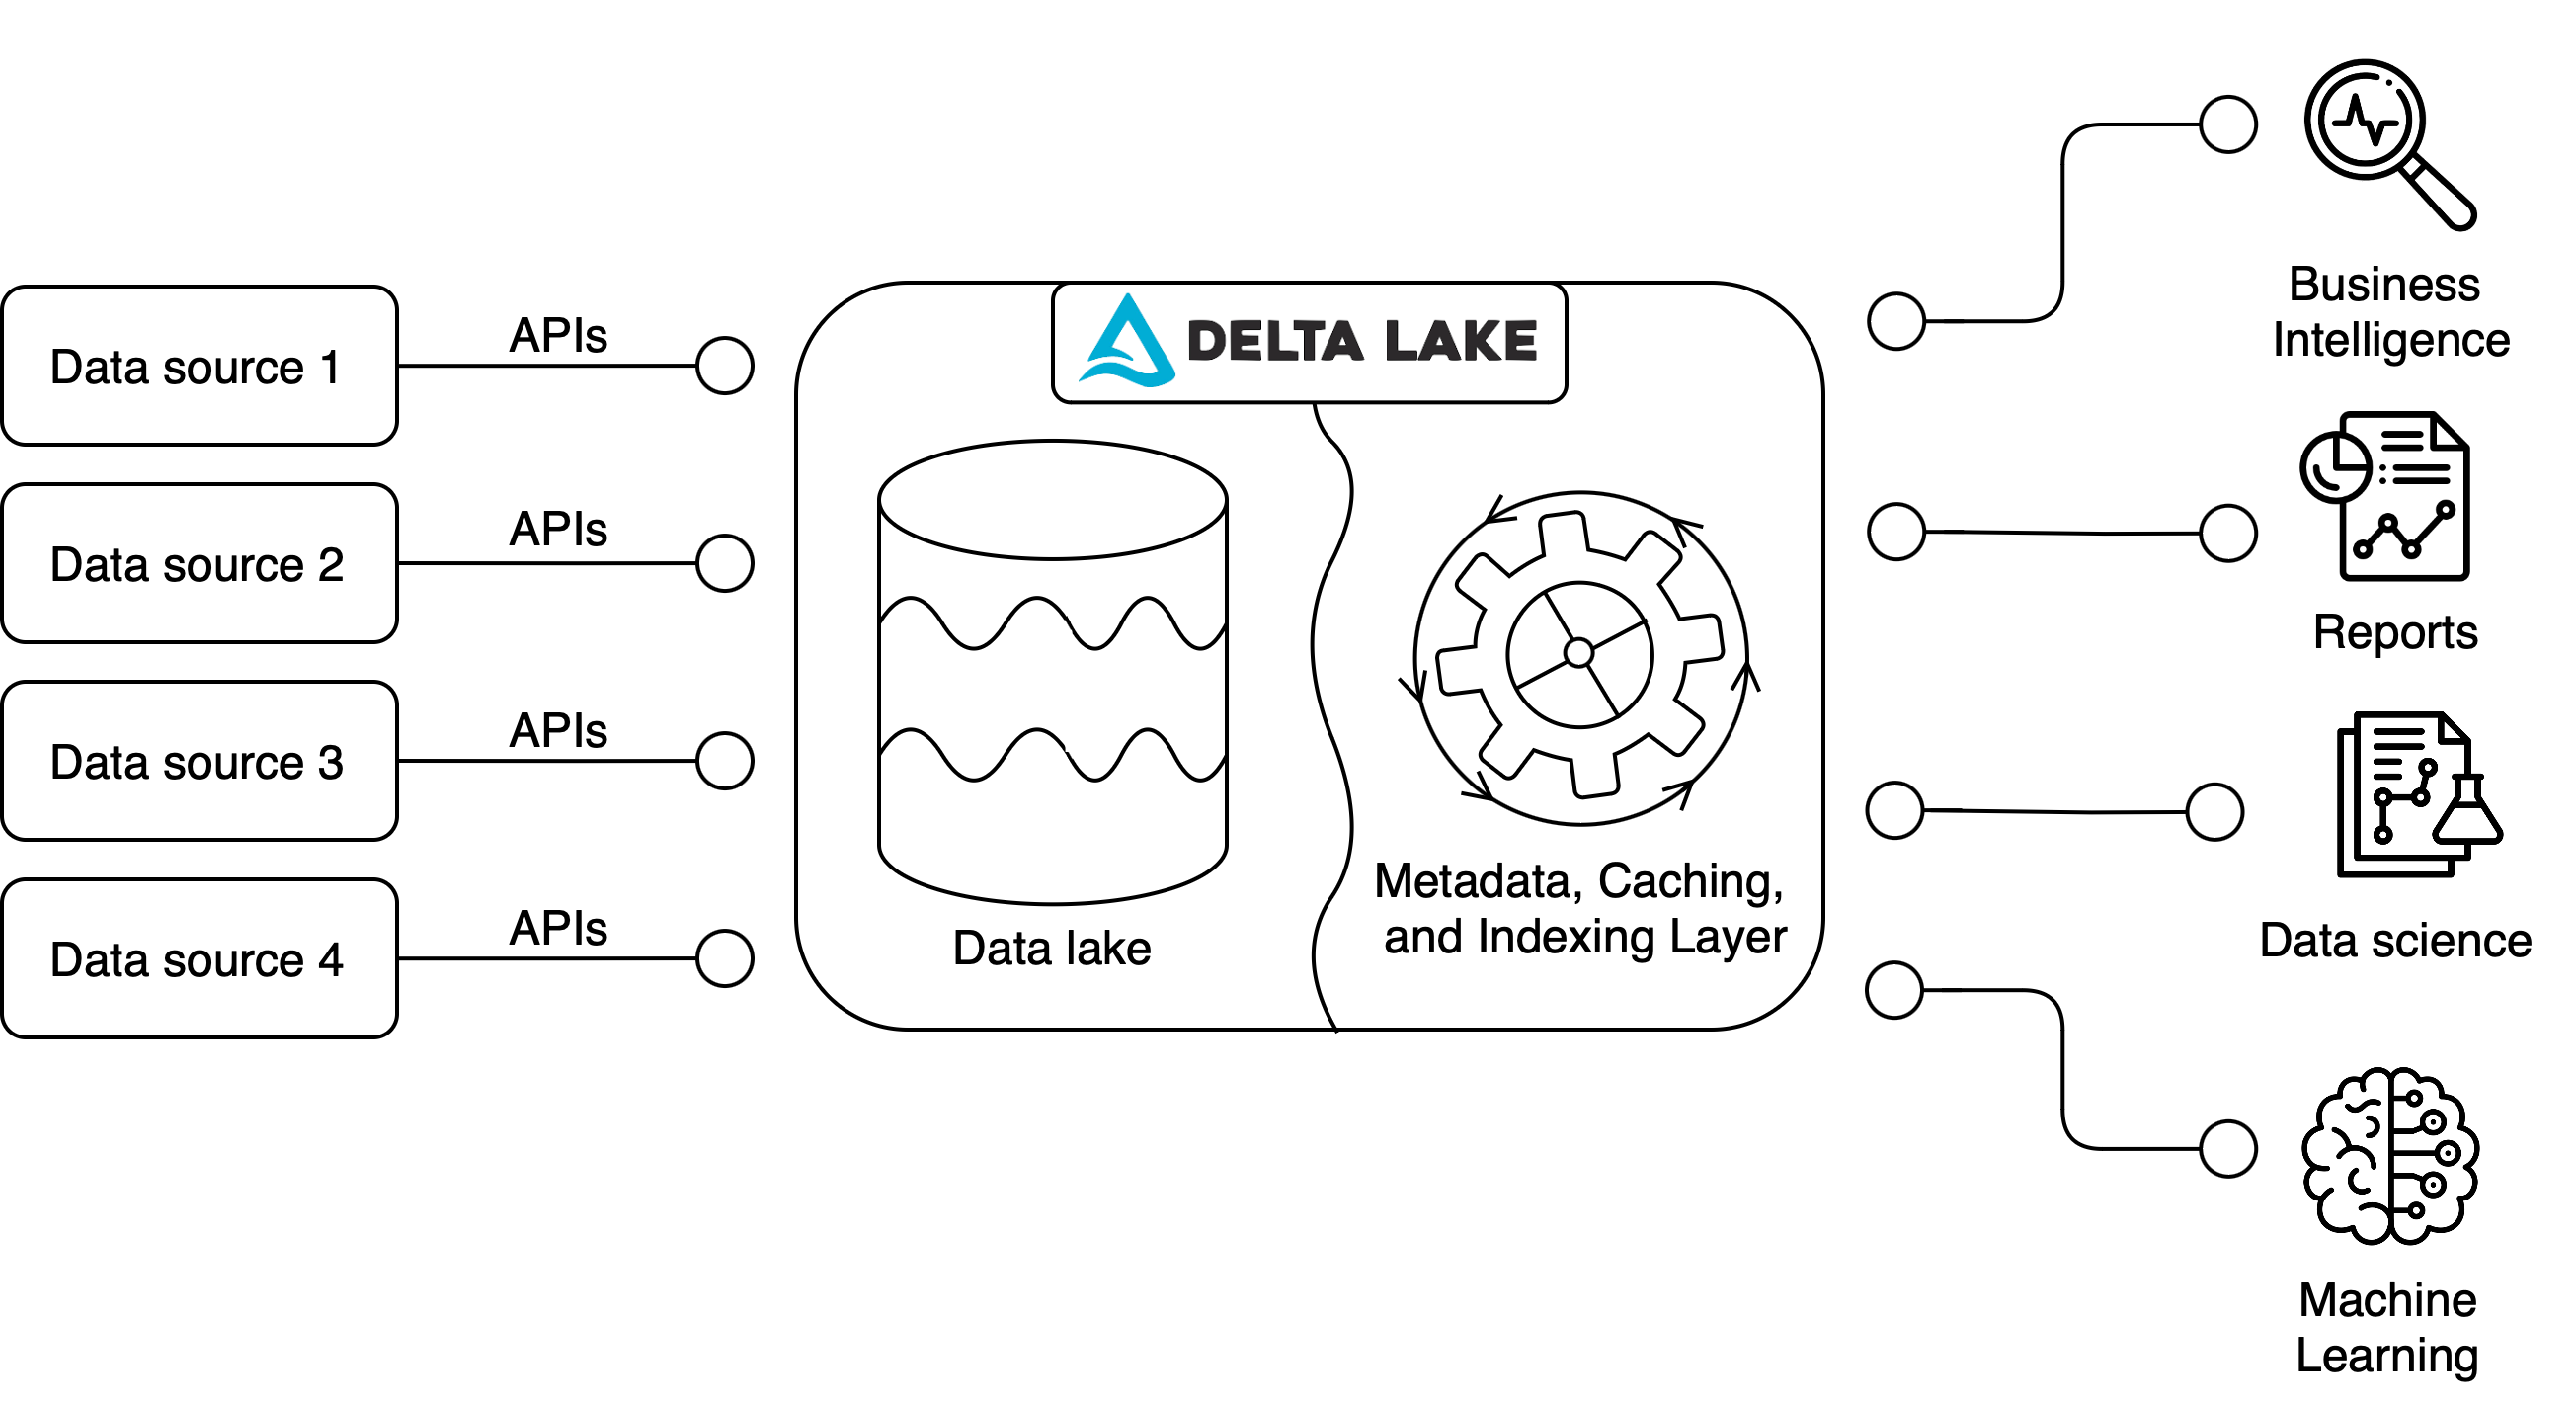
\includegraphics[width=\textwidth]{figures/2-background/DeltaLake_evolution-DeltaLake.png}
    \end{center}
    \caption{Delta lake system}
    \label{fig:DeltaLake}
\end{figure}

Figure \ref{fig:DeltaLake} shows a Delta Lake system \cite{armbrustDeltaLakeHighperformance2020}. The data lakehouse term was first introduced by Databricks in 2021 with their paper presented at \gls{CIDR} \cite{lakehouse2021}, while data lakehouse solutions already existed on the market, namely Apache Hudi \cite{rajaperumalUberEngineeringIncremental2017}, Apache Iceberg \cite{ApacheIcebergApache} and Delta Lake \cite{armbrustDeltaLakeHighperformance2020}. Data lakehouses combine the benefits of data warehouses and data lakes while simplifying the complexity of storing and accessing data in enterprise data architectures. This new architecture is based on an open-data format called parquet \cite{Parquet}, which is a column-based data file format. Data is saved in a data lake in the form of parquet files, then a management layer enables managing transactions, versioning, indexing, and other data management features. This enables data lakehouses to offer \gls{ACID} properties, similarly to data warehouses. 

Delta Lake is the technology that will be most used in this project. A Delta Lake Table (i.e. an instance of Delta Lake) works operating on a data lake containing parquet files and a transaction log. The transaction log records each operation, enabling versioning and recovery of previous versions (also called time travel). The data lake can be partitioned, e.g. using a date field, and this would make the Delta Lake table look as Figure \ref{fig:delta_table}. 

\begin{figure}
    \begin{center}
      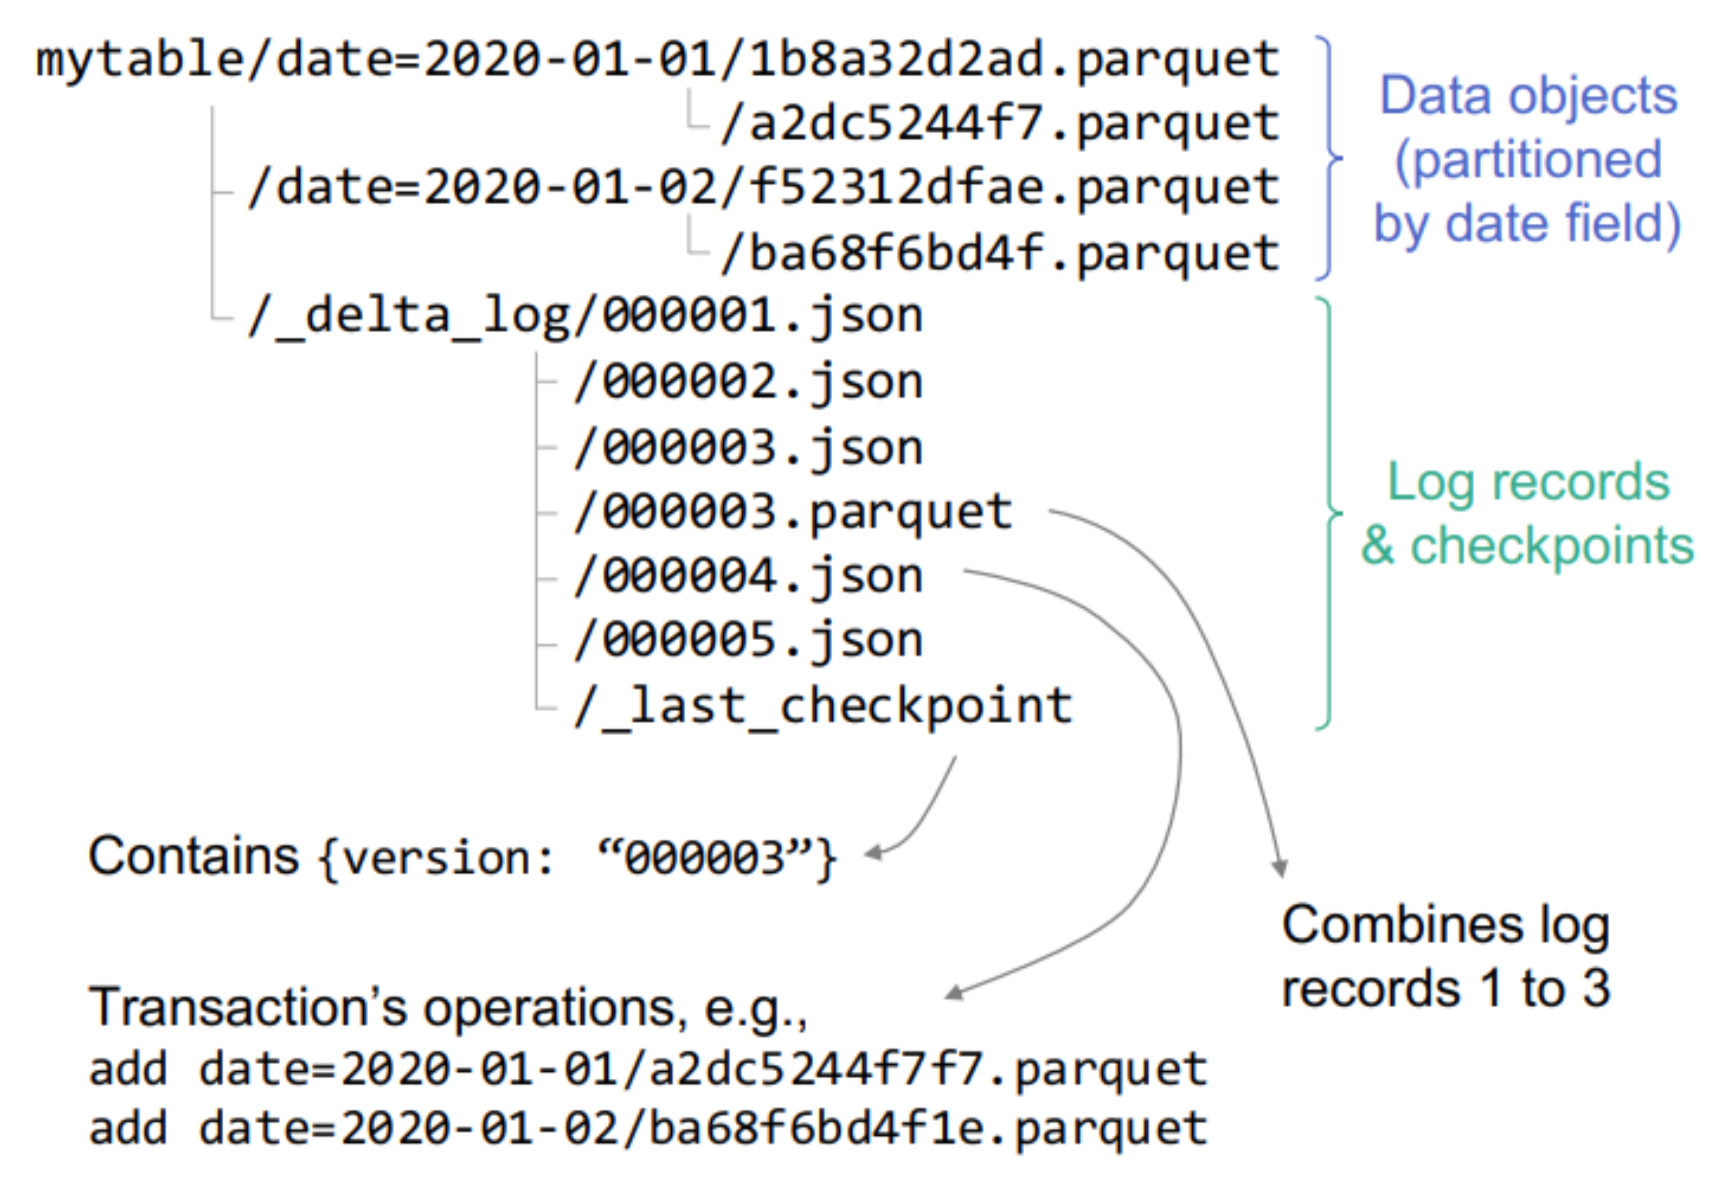
\includegraphics[width=\textwidth]{figures/2-background/delta_lake_table.png}
    \end{center}
    \caption{Delta lake table partitioned according to date field}
    \label{fig:delta_table}
\end{figure}

\subsection{Accessing Delta Lake}
\label{subsec:delta_lake_access}

The Delta Lake project is strictly related to Apache Spark, as Databricks (the company that developed Delta Lake) was built by the Spark developers \cite{zaharia2010spark} to offer big data management services around Spark. As of version 3.0 of Delta Lake, Delta Kernel was announced \cite{AnnouncingDeltaLake2023}, a Java library providing low-level access to Delta Lake, without needing to write the Delta Lake logic. While this move tried to standardize all accesses to Delta Lake under the Spark/Java environment, new ways to access the library had already been written since Delta Lake is an open-source project.

As early as April 2020, the Rust community started implementing a new interface to access Delta Lake written in Rust without \gls{JVM} dependencies. This library expanded even more the Delta Lake ecosystem, breaking the dependency between Delta Lake and Spark to perform operations on the data lakehouse. This worked particularly well considering that the data science community makes heavy use of Python and typically would avoid having \gls{JVM} dependencies. Being delta-rs written in Rust it makes the library highly compatible with Python since it can be easily wrapped and deployed as a Python library. This is perhaps the reason behind the fact that delta-rs can be simply installed in Python with the name "deltalake".